%%=============================================================================
%% Proof of concept ontwikkeling
%%=============================================================================

\chapter{\IfLanguageName{dutch}{Proof of Concept voorbereiding}{Proof of Concept Preparation}}%
\label{ch:proof of concept preparation}

In dit hoofdstuk wordt de proof of concept voorbereid, deze zal aan de requirements voldoen die in Hoofdstuk \ref{ch:requirements analyse} zijn opgesteld. Deze voorbereiding zal tot stand komen door middel van de vergaarde kennis uit het literatuuronderzoek en de interviews met de stakeholders.

\section{Nodige Netskope componenten}

In deze sectie worden de nodige Netskope componenten voor de proof of concept ontwikkeling besproken.

\subsection{Netskope Client}
De Netskope client is een applicatie die netwerkverkeer van eindgebruikersapparaten naar de Netskope Cloud stuurt, waar beveiligingsoplossingen zoals de Secure Web Gateway (SWG), Zero Trust Network Access (ZTNA) en Cloud Access Security Broker (CASB) worden toegepast. 

\vspace{2ex}

De client werkt via een forward proxy-mechanisme waarbij een SSL-tunnel wordt opgezet tussen het apparaat van de gebruiker en de Netskope proxy in de cloud. De te sturen applicaties en domeinen worden centraal geconfigureerd in de Netskope admin console en deze configuratie wordt automatisch verspreid en bijgewerkt op alle geïnstalleerde Clients. Tijdens de installatie worden alle benodigde CA-certificaten toegevoegd aan het systeem om correcte SSL-terminatie te waarborgen.
De Netskope client ondersteunt diverse besturingssystemen, waaronder Windows, macOS, Linux, Android, iOS en Chrome OS.

\vspace{2ex}

De uitrol kan plaatsvinden via verschillende methoden, zoals e-mailuitnodigingen, integratie met Identity Providers, of device management-platformen zoals Microsoft Intune, JAMF en VMware Workspace ONE. Na installatie zorgt de client voor zichtbaarheid en beleidsafdwinging op zowel beheerde als onbeheerde applicaties, ongeacht de locatie van de gebruiker~\autocite{Netskope2025-8}.

\subsection{Netskope Next Gen Secure Web Gateway (SWG)}
Een Secure Web Gateway (SWG) is ontwikkeld om webverkeer te beveiligen, ongewenste inhoud te filteren en gevoelige gegevens te beschermen. Netskope's Next-Gen SWG gaat verder door niet alleen webverkeer te beheren, maar ook uitgebreide zichtbaarheid en controle te bieden over het gebruik van cloud-applicaties en datastromen.
Deze oplossing richt zich specifiek op het detecteren van bedreigingen en het afdwingen van beveiligingsbeleid voor zowel web- als cloudomgevingen, met behoud van netwerkprestaties en betrouwbaarheid~\autocite{Netskope2025-3}.

\subsection{Netskope Cloud Access Security Broker (CASB)}
Een Cloud Access Security Broker (CASB) is een beveiligingsoplossing die zichtbaarheid, controle en bescherming biedt voor cloudapplicaties en -diensten. Netskope's CASB heeft diepgaande integraties met populaire cloudplatformen zoals Microsoft 365, Google Workspace, Salesforce, en Slack.

\vspace{2ex}

Het biedt real-time inzicht in gebruikersactiviteiten en datastromen binnen zowel persoonlijke als zakelijke accounts van cloudapplicaties zoals Dropbox, Box en GitHub~\autocite{Netskope2025-4}.

\subsection{Netskope Zero Trust Network Access (ZTNA)}
Zero Trust Network Access (ZTNA) is een beveiligingsframework dat gebruikers veilig verbindt met bedrijfsapplicaties op basis van het zero trust-model. Dit model gaat uit van het principe dat geen enkele gebruiker of apparaat automatisch wordt vertrouwd, ongeacht locatie of netwerk. 

\vspace{2ex}

Netskope’s ZTNA implementeert dit door toegang te beperken tot specifieke applicaties in plaats van volledige netwerktoegang te verlenen. In plaats van netwerktoegang biedt ZTNA alleen toegang tot specifieke, geautoriseerde applicaties. Dit voorkomt ongeautoriseerde laterale bewegingen binnen het netwerk, dit zijn een veelvoorkomende aanvalstechniek waarbij kwaadwillenden, na toegang te hebben verkregen tot één systeem, zich binnen een netwerk horizontaal verplaatsen naar andere systemen of applicaties. Bij traditionele VPN-oplossingen krijgt een gebruiker na authenticatie vaak brede toegang tot het bedrijfsnetwerk, waardoor een aanvaller die inloggegevens heeft gestolen, vrij kan bewegen tussen verschillende systemen. Dit kan leiden tot privilege escalation, gegevensdiefstal of het installeren van malware op kritieke systemen. Privilege escalation is het proces waarbij een aanvaller ongeautoriseerd hogere toegangsrechten verkrijgt binnen een systeem dan oorspronkelijk toegewezen, waardoor deze gevoelige gegevens kan benaderen of kritieke systeemfuncties kan manipuleren. 

\vspace{2ex}

ZTNA elimineert deze dreigingen door gebruikers alleen directe toegang te geven tot specifiek geautoriseerde applicaties, waardoor het onmogelijk wordt om tussen systemen te navigeren die niet expliciet zijn toegestaan. Een cloudgebaseerde ZTNA-broker verifieert de identiteit en beveiligingsstatus van gebruikers en apparaten voordat toegang wordt verleend. Bedrijfsapplicaties blijven onzichtbaar voor onbevoegde gebruikers, waardoor de digitale aanvalsoppervlakte aanzienlijk wordt verkleind. ZTNA elimineert traditionele kwetsbaarheden zoals inkomende netwerkverbindingen en biedt een veiliger alternatief door applicatiespecifieke toegang te combineren met een verbeterde gebruikerservaring en een gereduceerd risico op aanvallen~\autocite{Netskope2025-5}.

\subsection{Netskope Publisher}
Een Netskope publisher is een beveiligingsoplossing die remote werknemers toegang verleent tot private cloudapplicaties en -diensten zoals Microsoft 365, Google Workspace en Salesforce. Het werkt als een gateway tussen gebruikers en privé-applicaties, waardoor veilige en directe toegang mogelijk wordt zonder de noodzaak van traditionele VPN-oplossingen~\autocite{Netskope2025-6}~\autocite{Netskope2025-7}.

\section{Netskope architectuur}
In Figuur \ref{fig:poc-architecture} wordt de ontworpen architectuur voor de proof of concept afgebeeld. Hieronder wordt de architectuur per component uitgelegd.
\begin{figure}[h!]
    \centering
    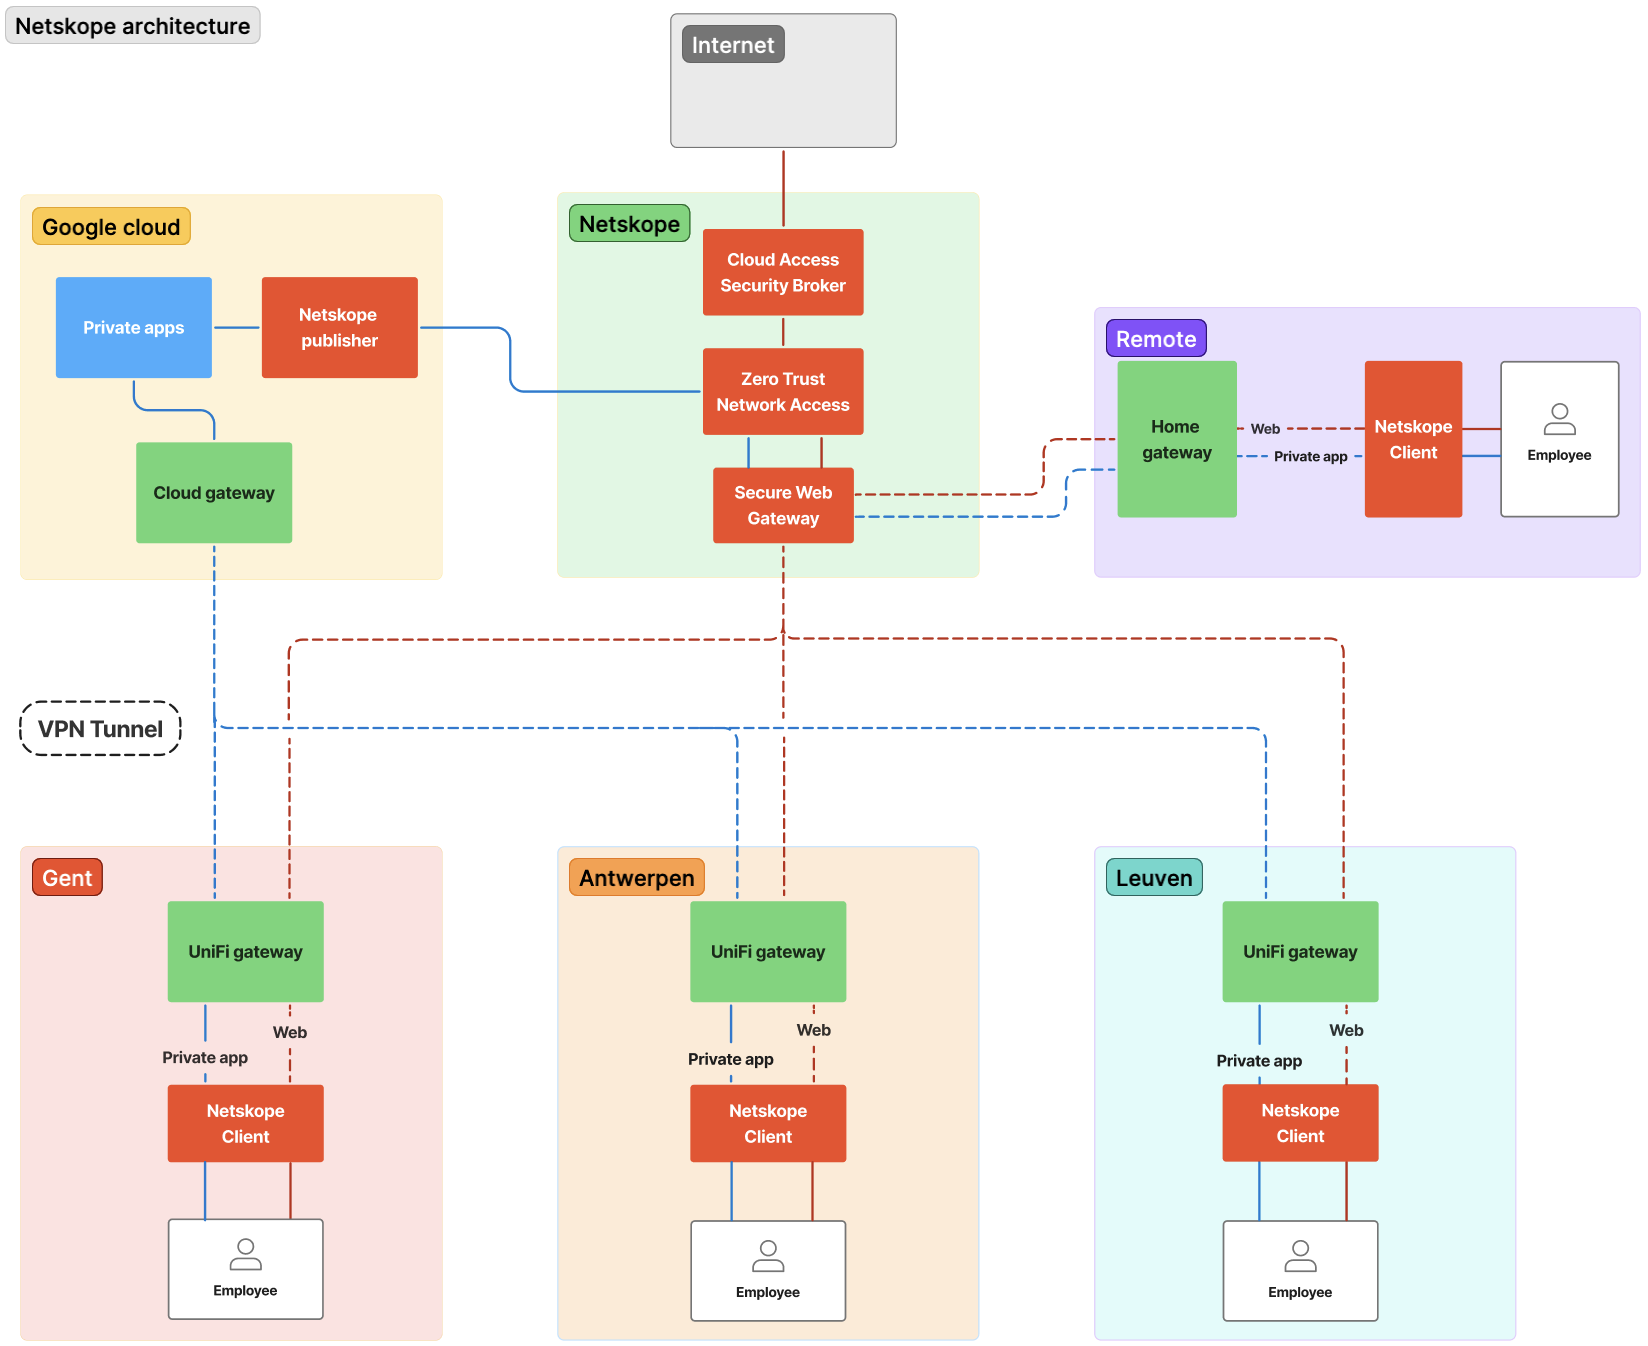
\includegraphics[width=\textwidth]{Netskope-architecture.png}
    \caption[Architectuur van de POC]{Architectuur van de proof of concept}
    \label{fig:poc-architecture}
\end{figure}
  
\subsection{Google Cloud}
Het bedrijf gebruikt Google Cloud als cloudprovider. Binnen Google Cloud worden de private apps van het bedrijf gehost. De Netskope Publisher wordt binnen de Google Cloud omgeving geplaatst om deze private apps remote beschikbaar te stellen. 

\subsection{Netskope Cloud}
De Netskope Cloud is de cloudomgeving van Netskope waarin de nodige Netskope componenten zich bevinden. De Netskope client verbindt met de cloud via een SSL tunnel.

\subsection{Gent, Antwerpen en Leuven}
Op elk van de sites van het bedrijf is er een UniFi gateway aanwezig, deze gateway heeft een IPSec tunnel naar de Google Cloud omgeving. Dit betekent dat we er voor kunnen kiezen om de private applicaties niet via Netskope te sturen maar via deze IPSec tunnel op basis van de gebruikerslocatie. Merk dus op dat het verkeer met betrekking tot de private applicaties niet wordt geëncrypteerd door Netskope, maar pas wordt geëncrypteerd op de gateway voor de IPSec tunnel.

\subsection{Remote}
Het verkeer van werknemers die op afstand werken zal dus wel volledig via Netskope worden gestuurd, aangezien de werknemers geen IPSec tunnel hebben naar de Google Cloud omgeving. Zoals je dan kan zien op de Figuur \ref{fig:poc-architecture} wordt het verkeer met betrekking tot de private apps wel geëncrypteerd door de Netskope client.

\section{Testgroep}
Voor een implementatie op deze schaal is een testgroep essentieel. Het bedrijf heeft meer dan 200 werknemers, dus is het risico op onvoorziene problemen en misconfiguraties te groot. Een testgroep zal er voor zorgen dat we incrementeel de tool kunnen uitwerken en uitrollen zonder dat de schade van misconfiguraties of onvoorziene problemen te groot is.

\vspace{2ex}

Het is belangrijk om een gestructureerde aanpak te hanteren bij de samenstelling van de testgroep, waarbij vertegenwoordigers uit verschillende afdelingen worden betrokken om zo een breed spectrum aan feedback te verzamelen. De testgroep dient idealiter te bestaan uit personen met variërende technische vaardigheden, van eindgebruikers tot IT-specialisten, zodat de SASE-implementatie vanuit diverse perspectieven kan worden beoordeeld.

\vspace{2ex}

De overgang van testfase naar volledige implementatie moet zorgvuldig worden gepland, met duidelijke mijlpalen en acceptatiecriteria die moeten worden bereikt voordat de SASE-oplossing in de gehele organisatie wordt uitge rold.

\section{Communicatie}
Bij de implementatie van een SASE-architectuur is heldere communicatie naar medewerkers van essentieel belang. Een SASE-oplossing, met zijn uitgebreide monitoring- en beveiligingsmogelijkheden, kan als privacy overschrijdend worden ervaren door werknemers die onvoldoende zijn geïnformeerd over het doel en de werking van deze technologie.

\subsection{Transparantie}
De sleutel tot succesvolle implementatie ligt bij transparante communicatie over waarom de organisatie kiest voor een SASE-architectuur. Het is belangrijk om duidelijk te maken dat het primaire doel niet het monitoren van medewerkers is, maar het beschermen van bedrijfsgegevens en het waarborgen van de veiligheid van de infrastructuur. Medewerkers moeten begrijpen dat deze implementatie hen ook beschermt tegen cyberdreigingen en dat het niet gaat om wantrouwen.

\subsection{Belangrijke communicatie-elementen}
Bij het communiceren over de SASE-implementatie moeten de volgende elementen aan bod komen:

\begin{itemize}
    \item \textbf{Doel en voordelen}: Verduidelijken waarom de organisatie kiest voor SASE en welke voordelen dit biedt voor zowel het bedrijf als de medewerkers.
    \item \textbf{Bereik van monitoring}: Transparant zijn over welke gegevens worden verzameld en wat er precies wordt gemonitord.
    \item \textbf{Privacy waarborgen}: De maatregelen beschrijven die worden genomen om de privacy van medewerkers te beschermen.
    \item \textbf{Procedure bij incidenten}: Medewerkers informeren over de procedure bij beveiligingsincidenten en hoe met hun gegevens wordt omgegaan.
    \item \textbf{Feedback mogelijkheden}: Kanalen creëren waar medewerkers vragen kunnen stellen of zorgen kunnen uiten over de implementatie.
\end{itemize}

\subsection{Aandacht voor weerstand}
Het is normaal dat er enige weerstand bestaat tegen veranderingen, zeker wanneer die raken aan privacy-gevoelige aspecten. Door proactief te communiceren en medewerkers te betrekken bij de implementatie, kan deze weerstand worden verminderd. Luisteren naar zorgen van medewerkers en deze serieus nemen is hier dus essentieel.

\vspace{2ex}

Door een goed communicatieplan te ontwikkelen en uit te voeren, wordt de acceptatie van de SASE-oplossing bevorderd en worden misverstanden voorkomen. Dit draagt bij aan het succes van de implementatie en zorgt voor een betere beveiliging van de digitale omgeving van de organisatie, zonder dat medewerkers het gevoel krijgen dat hun privacy wordt geschonden.
